\section{XMPush\-Button  Class Reference}
\label{classXMPushButton}\index{XMPushButton@{XMPush\-Button}}
{\tt \#include $<$XMPushbutton.h$>$}

Inheritance diagram for XMPush\-Button::\begin{figure}[H]
\begin{center}
\leavevmode
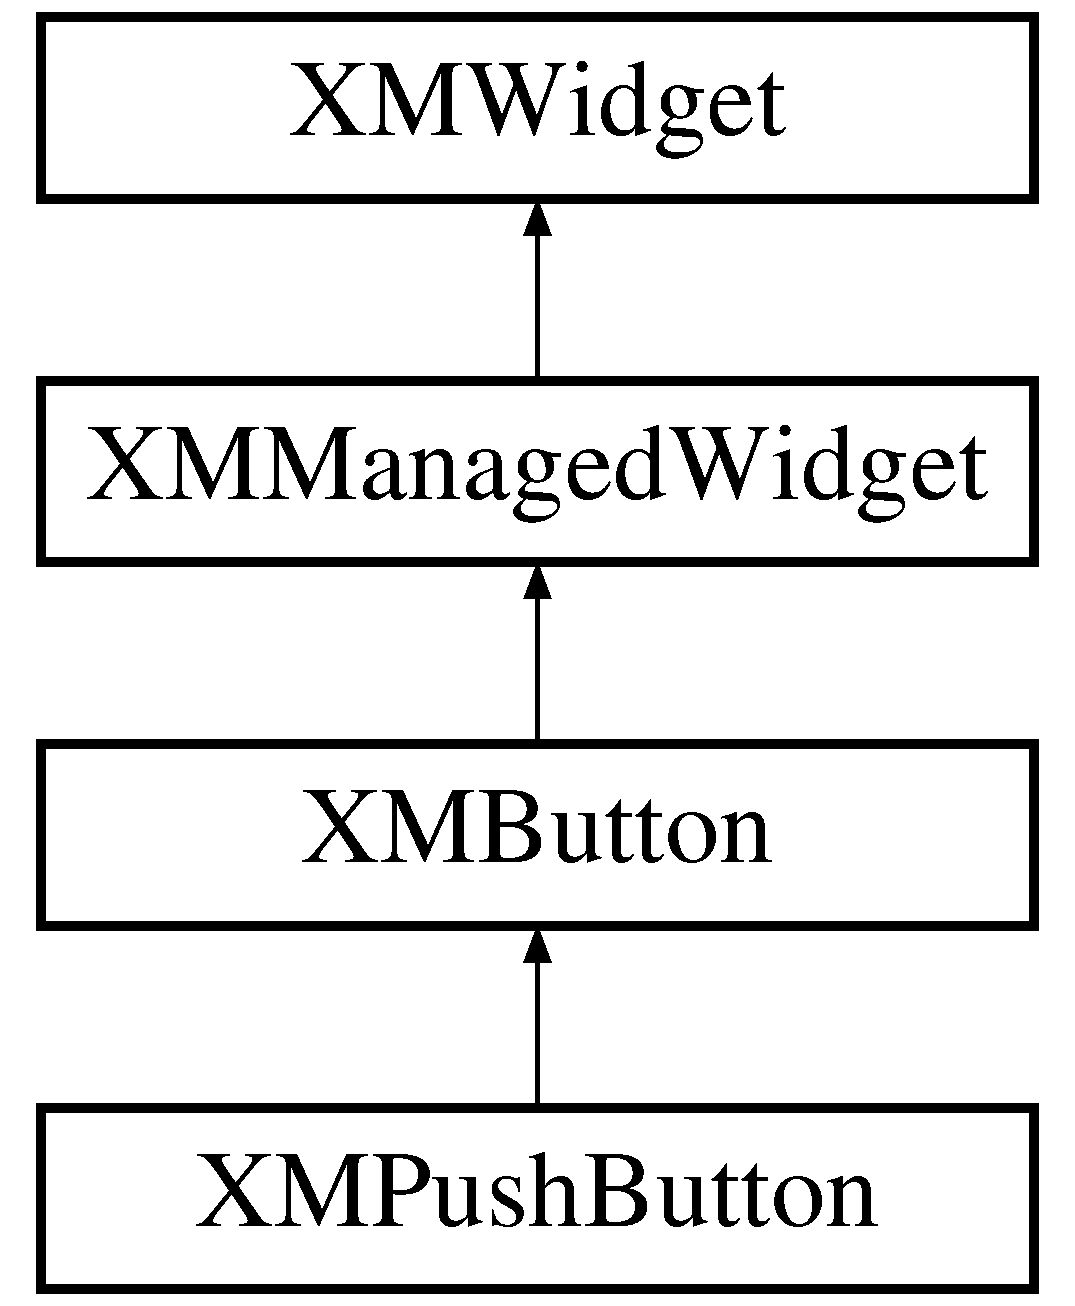
\includegraphics[height=4cm]{classXMPushButton}
\end{center}
\end{figure}
\subsection*{Public Methods}
\begin{CompactItemize}
\item 
{\bf XMPush\-Button} (char $\ast$n, Widget parent, void($\ast$cb)({\bf XMWidget} $\ast$, Xt\-Pointer, Xt\-Pointer)=NULL, Xt\-Pointer cd=NULL)
\item 
{\bf XMPush\-Button} (char $\ast$n, {\bf XMWidget} \&parent, void($\ast$cb)({\bf XMWidget} $\ast$, Xt\-Pointer, Xt\-Pointer)=NULL, Xt\-Pointer cd=NULL)
\item 
{\bf XMPush\-Button} (Widget w)
\item 
{\bf Callback\_\-data} $\ast$ {\bf Add\-Callback} (void($\ast$cb)({\bf XMWidget} $\ast$, Xt\-Pointer, Xt\-Pointer)=NULL, Xt\-Pointer cd=NULL)
\end{CompactItemize}


\subsection{Constructor \& Destructor Documentation}
\index{XMPushButton@{XMPush\-Button}!XMPushButton@{XMPushButton}}
\index{XMPushButton@{XMPushButton}!XMPushButton@{XMPush\-Button}}
\subsubsection{\setlength{\rightskip}{0pt plus 5cm}XMPush\-Button::XMPush\-Button (char $\ast$ {\em n}, Widget {\em parent}, void($\ast$ {\em cb})({\bf XMWidget} $\ast$, Xt\-Pointer, Xt\-Pointer) = NULL, Xt\-Pointer {\em cd} = NULL)\hspace{0.3cm}{\tt  [inline]}}\label{classXMPushButton_a0}




Definition at line 377 of file XMPushbutton.h.

References XMWidget::Add\-Callback(), and XMButton::Enable().\index{XMPushButton@{XMPush\-Button}!XMPushButton@{XMPushButton}}
\index{XMPushButton@{XMPushButton}!XMPushButton@{XMPush\-Button}}
\subsubsection{\setlength{\rightskip}{0pt plus 5cm}XMPush\-Button::XMPush\-Button (char $\ast$ {\em n}, {\bf XMWidget} \& {\em parent}, void($\ast$ {\em cb})({\bf XMWidget} $\ast$, Xt\-Pointer, Xt\-Pointer) = NULL, Xt\-Pointer {\em cd} = NULL)\hspace{0.3cm}{\tt  [inline]}}\label{classXMPushButton_a1}




Definition at line 387 of file XMPushbutton.h.

References XMWidget::Add\-Callback(), and XMButton::Enable().\index{XMPushButton@{XMPush\-Button}!XMPushButton@{XMPushButton}}
\index{XMPushButton@{XMPushButton}!XMPushButton@{XMPush\-Button}}
\subsubsection{\setlength{\rightskip}{0pt plus 5cm}XMPush\-Button::XMPush\-Button (Widget {\em w})\hspace{0.3cm}{\tt  [inline]}}\label{classXMPushButton_a2}




Definition at line 397 of file XMPushbutton.h.

\subsection{Member Function Documentation}
\index{XMPushButton@{XMPush\-Button}!AddCallback@{AddCallback}}
\index{AddCallback@{AddCallback}!XMPushButton@{XMPush\-Button}}
\subsubsection{\setlength{\rightskip}{0pt plus 5cm}{\bf Callback\_\-data}$\ast$ XMPush\-Button::Add\-Callback (void($\ast$ {\em cb})({\bf XMWidget} $\ast$, Xt\-Pointer, Xt\-Pointer) = NULL, Xt\-Pointer {\em cd} = NULL)\hspace{0.3cm}{\tt  [inline]}}\label{classXMPushButton_a3}




Definition at line 400 of file XMPushbutton.h.

References XMWidget::Add\-Callback().

The documentation for this class was generated from the following file:\begin{CompactItemize}
\item 
{\bf XMPushbutton.h}\end{CompactItemize}
